

%----------------------------------------------------------------------
\begin{frame}[fragile]
  \frametitle{Follow-up and rates}
  \begin{itemize}[<+->]
  \item In follow-up studies we estimate rates from:

    \begin{itemize}[<+->]
    \item $D$ --- events, deaths
    \item $Y$ --- person-years
    \item $\hat\lambda = D/Y$ rates
    \item \ldots empirical counterpart of intensity --- \textbf{estimate}
    \end{itemize}

  \item Rates differ between persons.
  \item Rates differ \textcolor{blue}{within} persons:

    \begin{itemize}[<+->]
    \item By age
    \item By calendar time
    \item By disease duration
    \item \ldots
    \end{itemize}

  \item Multiple timescales.
  \item Multiple states (little boxes --- later)
  \end{itemize}

\end{frame}

%----------------------------------------------------------------------
\begin{frame}[fragile]
  \frametitle{Examples: stratification by age}
If follow-up is rather short, age at entry is OK for age-stratification.

If follow-up is long, use stratification by categories of\\
\textbf{current age}, both for:

No. of events, $D$, and Risk time, $Y$.

\setlength{\unitlength}{1pt}
\begin{center}
\begin{picture}(210,70)(0,75)
%\scriptsize
\thicklines
 \put(  0,80){\makebox(0,0)[r]{Age-scale}}
 \put( 50,80){\line(1,0){150}}
 \put( 50,80){\line(0,1){5}}
 \put(100,80){\line(0,1){5}}
 \put(150,80){\line(0,1){5}}
 \put(200,80){\line(0,1){5}}
 \put( 50,77){\makebox(0,0)[t]{35}}
 \put(100,77){\makebox(0,0)[t]{40}}
 \put(150,77){\makebox(0,0)[t]{45}}
 \put(200,77){\makebox(0,0)[t]{50}}

 \put(  0,115){\makebox(0,0)[r]{Follow-up}}

 \put( 80,105){\makebox(0,0)[r]{\small Two}}
 \put( 90,105){\line(1,0){87}}
 \put( 90,100){\line(0,1){10}}
 \put(100,100){\line(0,1){10}}
 \put(150,100){\line(0,1){10}}
 \put(180,105){\circle{6}}
 \put( 95,110){\makebox(0,0)[b]{1}}
 \put(125,110){\makebox(0,0)[b]{5}}
 \put(165,110){\makebox(0,0)[b]{3}}

 \put( 50,130){\makebox(0,0)[r]{\small One}}
 \put( 60,130){\line(1,0){70}}
 \put( 60,125){\line(0,1){10}}
 \put(100,125){\line(0,1){10}}
 \put(130,130){\circle*{6}}
 \put( 80,135){\makebox(0,0)[b]{4}}
 \put(115,135){\makebox(0,0)[b]{3}}
\end{picture}
\end{center}
\pause
--- assuming a constant rate $\lambda$ throughout. 
\end{frame}

%----------------------------------------------------------------------
\begin{frame}[fragile]
  \frametitle{Representation of follow-up data}
A cohort or follow-up study records:\\
\textbf{Events} and \textbf{Risk time}.

The outcome is thus \textbf{bivariate}: $(d,y)$

Follow-up \textbf{data} for each individual must therefore have (at least) three variables:
\begin{center}
\begin{tabular}{lll}
\toprule
Date of entry  & \verb+entry+ & date variable\\
Date of exit   & \verb+exit+  & date variable\\
Status at exit & \verb+fail+  & indicator (0/1)\\
\bottomrule
\end{tabular}
\end{center}
Specific for each \textbf{type} of outcome.

\end{frame}

%----------------------------------------------------------------------
\begin{frame}[fragile]

\setlength{\unitlength}{1pt}
\begin{center}
\begin{picture}(250,40)
%\scriptsize
\thicklines
\onslide<1->{
\textcolor{blue}{
 \put( 10,35){\line(1,0){230}}
 \put( 10,32){\line(0,1){6}}
 \put(240,32){\line(0,1){6}}
 %\put(240,35){\circle{6}}
 \put(120,37){\makebox(0,0)[cb]{$y$}}
 }

 \put(240,41){\makebox(0,0)[cb]{$d$}}
 \put( 10,20){\makebox(0,0)[c]{$t_0$}}
}
\onslide<2->{\put( 80,20){\makebox(0,0)[c]{$t_1$}}}
\onslide<2->{\put(180,20){\makebox(0,0)[c]{$t_2$}}}
 \put(240,20){\makebox(0,0)[c]{$t_\text{x}$}}
\onslide<2->{\textcolor{red}{
 \put( 10, 5){\line(1,0){230}}
 \put( 10, 2){\line(0,1){6}}
 \put( 80, 2){\line(0,1){6}}
 \put(180, 2){\line(0,1){6}}
 \put(240, 2){\line(0,1){6}}
 %\put(240, 5){\circle{6}}
 \put( 45, 1){\makebox(0,0)[ct]{$y_1$}}
 \put(120, 1){\makebox(0,0)[ct]{$y_2$}}
 \put(210, 1){\makebox(0,0)[ct]{$y_3$}}
 } }
\end{picture}
\end{center}
\vspace*{-1em}
\begin{align*}
  & \hspace*{-1ex} \text{Probability}
& & \hspace*{-1ex} \text{log-Likelihood} \\[1ex]
  & \hspace*{-1ex} \textcolor{blue}{\operatorname{P}(\text{\textcolor{black}{$d$} at $t_\text{x}$} | \text{entry $t_0$})}
  & \qquad
  & \hspace*{-1ex} d\,\textcolor{blue}{\log(\lambda) - \lambda}y\\[1ex]
  &\onslide<3->{\textcolor{red}{ = \operatorname{P}(\text{surv $t_0\rightarrow \textcolor{red}{t_1}$} | \text{entry $t_0$}) } }
& &\onslide<6->{\textcolor{red}{\,=\,}0\,\textcolor{red}{ \log(\lambda) - \lambda} y_1}\\
  &\onslide<4->{\textcolor{red}{\times \operatorname{P}(\text{surv $\textcolor{red}{t_1}\rightarrow \textcolor{red}{t_2}$} | \text{entry \textcolor{red}{$t_1$}})} }
& &\onslide<6->{\textcolor{red}{\,+\,}0\,\textcolor{red}{ \log(\lambda) - \lambda} y_2}\\
  &\onslide<5->{\textcolor{red}{\times \operatorname{P}(\text{$d$ at $t_\text{x}$} | \text{entry \textcolor{red}{$t_2$}}) } }
& &\onslide<6->{\textcolor{red}{\,+\,}d\,\textcolor{red}{ \log(\lambda) - \lambda} y_3}
\end{align*}

\end{frame}

%----------------------------------------------------------------------
\begin{frame}[fragile]

\setlength{\unitlength}{1pt}
\begin{center}
\begin{picture}(250,40)
%\scriptsize
\thicklines
\onslide<1->{
\textcolor{blue}{
 \put( 10,35){\line(1,0){227}}
 \put( 10,32){\line(0,1){6}}
 %\put(240,32){\line(0,1){6}}
 \put(120,37){\makebox(0,0)[cb]{$y$}}
 }
 \put(240,35){\circle{6}}

 \put(240,41){\makebox(0,0)[cb]{$d=0$}}
 \put( 10,20){\makebox(0,0)[c]{$t_0$}}
}
\onslide<1->{\put( 80,20){\makebox(0,0)[c]{$t_1$}}}
\onslide<1->{\put(180,20){\makebox(0,0)[c]{$t_2$}}}
 \put(240,20){\makebox(0,0)[c]{$t_\text{x}$}}
\onslide<1->{\textcolor{red}{
 \put( 10, 5){\line(1,0){227}}
 \put( 10, 2){\line(0,1){6}}
 \put( 80, 2){\line(0,1){6}}
 \put(180, 2){\line(0,1){6}}
 %\put(240, 2){\line(0,1){6}}
 \put( 45, 1){\makebox(0,0)[ct]{$y_1$}}
 \put(120, 1){\makebox(0,0)[ct]{$y_2$}}
 \put(210, 1){\makebox(0,0)[ct]{$y_3$}}
 } }
 \put(240, 5){\circle{6}}
\end{picture}
\end{center}
\vspace*{-1em}
\begin{align*}
  & \hspace*{-1ex} \text{Probability}
& & \hspace*{-1ex} \text{log-Likelihood} \\[1ex]
  & \hspace*{-1ex} \textcolor{blue}{\operatorname{P}(\text{surv $t_0 \rightarrow t_\text{x}$} | \text{entry $t_0$})}
  & \qquad
  & \hspace*{-1ex} 0\,\textcolor{blue}{\log(\lambda) - \lambda }y\\[1ex]
  &\onslide<1->{\textcolor{red}{ = \operatorname{P}(\text{surv $t_0\rightarrow \textcolor{red}{t_1}$} | \text{entry $t_0$}) } }
& &\onslide<1->{\textcolor{red}{\,=\,}0\,\textcolor{red}{ \log(\lambda) - \lambda} y_1}\\
  &\onslide<1->{\textcolor{red}{\times \operatorname{P}(\text{surv $\textcolor{red}{t_1}\rightarrow \textcolor{red}{t_2}$} | \text{entry \textcolor{red}{$t_1$}})} }
& &\onslide<1->{\textcolor{red}{\,+\,}0\,\textcolor{red}{ \log(\lambda) - \lambda} y_2}\\
  &\onslide<1->{\textcolor{red}{\times \operatorname{P}(\text{surv $t_2\rightarrow t_\text{x}$} | \text{entry \textcolor{red}{$t_2$}}) } }
& &\onslide<1->{\textcolor{red}{\,+\,}0\,\textcolor{red}{ \log(\lambda) - \lambda} y_3}
\end{align*}

\end{frame}

%----------------------------------------------------------------------
\begin{frame}[fragile]

\setlength{\unitlength}{1pt}
\begin{center}
\begin{picture}(250,40)
%\scriptsize
\thicklines
\onslide<1->{
\textcolor{blue}{
 \put( 10,35){\line(1,0){227}}
 \put( 10,32){\line(0,1){6}}
 %\put(240,32){\line(0,1){6}}
 \put(120,37){\makebox(0,0)[cb]{$y$}}
 }
 \put(240,35){\circle*{6}}

 \put(240,41){\makebox(0,0)[cb]{$d=1$}}
 \put( 10,20){\makebox(0,0)[c]{$t_0$}}
}
\onslide<1->{\put( 80,20){\makebox(0,0)[c]{$t_1$}}}
\onslide<1->{\put(180,20){\makebox(0,0)[c]{$t_2$}}}
 \put(240,20){\makebox(0,0)[c]{$t_\text{x}$}}
\onslide<1->{\textcolor{red}{
 \put( 10, 5){\line(1,0){227}}
 \put( 10, 2){\line(0,1){6}}
 \put( 80, 2){\line(0,1){6}}
 \put(180, 2){\line(0,1){6}}
 %\put(240, 2){\line(0,1){6}}
 \put( 45, 1){\makebox(0,0)[ct]{$y_1$}}
 \put(120, 1){\makebox(0,0)[ct]{$y_2$}}
 \put(210, 1){\makebox(0,0)[ct]{$y_3$}}
 } }
 \put(240, 5){\circle*{6}}
\end{picture}
\end{center}
\vspace*{-1em}
\begin{align*}
  & \hspace*{-1ex} \text{Probability}
& & \hspace*{-1ex} \text{log-Likelihood} \\[1ex]
  & \hspace*{-1ex} \textcolor{blue}{\operatorname{P}(\text{event at $t_\text{x}$} | \text{entry $t_0$})}
  & \qquad
  & \hspace*{-1ex} 1\,\textcolor{blue}{\log(\lambda) - \lambda} y\\[1ex]
  &\onslide<1->{\textcolor{red}{ = \operatorname{P}(\text{surv $t_0\rightarrow \textcolor{red}{t_1}$} | \text{entry $t_0$}) } }
& &\onslide<1->{\textcolor{red}{\,=\,}0\,\textcolor{red}{ \log(\lambda) - \lambda} y_1}\\
  &\onslide<1->{\textcolor{red}{\times \operatorname{P}(\text{surv $\textcolor{red}{t_1}\rightarrow \textcolor{red}{t_2}$} | \text{entry \textcolor{red}{$t_1$}})} }
& &\onslide<1->{\textcolor{red}{\,+\,}0\,\textcolor{red}{ \log(\lambda) - \lambda} y_2}\\
  &\onslide<1->{\textcolor{red}{\times \operatorname{P}(\text{event at $t_\text{x}$} | \text{entry \textcolor{red}{$t_2$}}) } }
& &\onslide<1->{\textcolor{red}{\,+\,}1\,\textcolor{red}{ \log(\lambda) - \lambda} y_3}
\end{align*}

\end{frame}

%----------------------------------------------------------------------
\begin{frame}[fragile]

\setlength{\unitlength}{1pt}
\begin{center}
\begin{picture}(250,40)
%\scriptsize
\thicklines
\onslide<1->{
\textcolor{blue}{
 \put( 10,35){\line(1,0){230}}
 \put( 10,32){\line(0,1){6}}
 \put(240,32){\line(0,1){6}}
 %\put(240,35){\circle{6}}
 \put(120,37){\makebox(0,0)[cb]{$y$}}
 }

 \put(240,41){\makebox(0,0)[cb]{$d$}}
 \put( 10,20){\makebox(0,0)[c]{$t_0$}}
}
\onslide<2->{\put( 80,20){\makebox(0,0)[c]{$t_1$}}}
\onslide<2->{\put(180,20){\makebox(0,0)[c]{$t_2$}}}
 \put(240,20){\makebox(0,0)[c]{$t_\text{x}$}}
\onslide<2->{\textcolor{red}{
 \put( 10, 5){\line(1,0){230}}
 \put( 10, 2){\line(0,1){6}}
 \put( 80, 2){\line(0,1){6}}
 \put(180, 2){\line(0,1){6}}
 \put(240, 2){\line(0,1){6}}
 %\put(240, 5){\circle{6}}
 \put( 45, 1){\makebox(0,0)[ct]{$y_1$}}
 \put(120, 1){\makebox(0,0)[ct]{$y_2$}}
 \put(210, 1){\makebox(0,0)[ct]{$y_3$}}
 } }
\end{picture}
\end{center}
\vspace*{-1em}
\begin{align*}
  & \hspace*{-1ex} \text{Probability}
& & \hspace*{-1ex} \text{log-Likelihood} \\[1ex]
  & \hspace*{-1ex} \textcolor{blue}{\operatorname{P}(\text{\textcolor{black}{$d$} at $t_\text{x}$} | \text{entry $t_0$})}
  & \qquad
  & \hspace*{-1ex} d\,\textcolor{blue}{\log(\lambda) - \lambda}y\\[1ex]
  &\onslide<2->{\textcolor{red}{ = \operatorname{P}(\text{surv $t_0\rightarrow \textcolor{red}{t_1}$} | \text{entry $t_0$}) } }
& &\onslide<2->{\textcolor{red}{\,=\,}0\,\textcolor{red}{ \log(\lambda) - \lambda} y_1}\\
  &\onslide<2->{\textcolor{red}{\times \operatorname{P}(\text{surv $\textcolor{red}{t_1}\rightarrow \textcolor{red}{t_2}$} | \text{entry \textcolor{red}{$t_1$}})} }
& &\onslide<2->{\textcolor{red}{\,+\,}0\,\textcolor{red}{ \log(\lambda) - \lambda} y_2}\\
  &\onslide<2->{\textcolor{red}{\times \operatorname{P}(\text{$d$ at $t_\text{x}$} | \text{entry \textcolor{red}{$t_2$}}) } }
& &\onslide<2->{\textcolor{red}{\,+\,}d\,\textcolor{red}{ \log(\lambda) - \lambda} y_3}
\end{align*}

\end{frame}

%----------------------------------------------------------------------
\begin{frame}[fragile]

\setlength{\unitlength}{1pt}
\begin{center}
\begin{picture}(250,40)
%\scriptsize
\thicklines
\onslide<1->{
\textcolor{blue}{
 \put( 10,35){\line(1,0){230}}
 \put( 10,32){\line(0,1){6}}
 \put(240,32){\line(0,1){6}}
 %\put(240,35){\circle{6}}
 \put(120,37){\makebox(0,0)[cb]{$y$}}
 }

 \put(240,41){\makebox(0,0)[cb]{$d$}}
 \put( 10,20){\makebox(0,0)[c]{$t_0$}}
}
\onslide<1->{\put( 80,20){\makebox(0,0)[c]{$t_1$}}}
\onslide<1->{\put(180,20){\makebox(0,0)[c]{$t_2$}}}
 \put(240,20){\makebox(0,0)[c]{$t_\text{x}$}}
\onslide<1->{\textcolor{red}{
 \put( 10, 5){\line(1,0){230}}
 \put( 10, 2){\line(0,1){6}}
 \put( 80, 2){\line(0,1){6}}
 \put(180, 2){\line(0,1){6}}
 \put(240, 2){\line(0,1){6}}
 %\put(240, 5){\circle{6}}
 \put( 45, 1){\makebox(0,0)[ct]{$y_1$}}
 \put(120, 1){\makebox(0,0)[ct]{$y_2$}}
 \put(210, 1){\makebox(0,0)[ct]{$y_3$}}
 } }
\end{picture}
\end{center}
\vspace*{-1em}
\begin{align*}
  & \hspace*{-1ex} \text{Probability}
& & \hspace*{-1ex} \text{log-Likelihood} \\[1ex]
  & \hspace*{-1ex} \textcolor{blue}{\operatorname{P}(\text{\textcolor{black}{$d$} at $t_\text{x}$} | \text{entry $t_0$})}
  & \qquad
  & \hspace*{-1ex} d\,\textcolor{blue}{\log(\lambda) - \lambda}y\\[1ex]
  &\onslide<1->{\textcolor{red}{ = \operatorname{P}(\text{surv $t_0\rightarrow \textcolor{red}{t_1}$} | \text{entry $t_0$}) } }
& &\onslide<1->{\textcolor{red}{\,=\,}0\,\textcolor{red}{ \log(\lambda_{\textcolor{forestgreen}{1}}) 
                                                             - \lambda_{\textcolor{forestgreen}{1}}} y_1}\\
  &\onslide<1->{\textcolor{red}{\times \operatorname{P}(\text{surv $\textcolor{red}{t_1}\rightarrow \textcolor{red}{t_2}$} | \text{entry \textcolor{red}{$t_1$}})} }
& &\onslide<1->{\textcolor{red}{\,+\,}0\,\textcolor{red}{ \log(\lambda_{\textcolor{forestgreen}{2}})
                                                             - \lambda_{\textcolor{forestgreen}{2}}} y_2}\\
  &\onslide<1->{\textcolor{red}{\times \operatorname{P}(\text{$d$ at $t_\text{x}$} | \text{entry \textcolor{red}{$t_2$}}) } }
& &\onslide<1->{\textcolor{red}{\,+\,}d\,\textcolor{red}{ \log(\lambda_{\textcolor{forestgreen}{3}})
                                                             - \lambda_{\textcolor{forestgreen}{3}}} y_3}
\end{align*}
\pause
--- allows different rates ($\lambda_{\textcolor{forestgreen}{i}}$) in each interval
\end{frame}

%----------------------------------------------------------------------
\begin{frame}
  \frametitle{Dividing time into bands:} 

  If we want to compute $D$ and $Y$ in intervals on some timescale we
  must decide on:

\pause
\textbf{Origin:} The date where the time scale is $0$: \pause
  \begin{itemize}
  \item Age --- $0$ at date of birth
  \item Disease duration --- $0$ at date of diagnosis
  \item Occupation exposure --- $0$ at date of hire
  \end{itemize}

\pause
\textbf{Intervals:} How should it be subdivided:
 \begin{itemize}
  \item 1-year classes? 5-year classes?
  \item Equal length?
  \end{itemize}

\pause
\textbf{Aim:} Separate rate in each interval

\end{frame}

%----------------------------------------------------------------------
\begin{frame}[fragile]
  \frametitle{Example: cohort with 3 persons:}
\small
\renewcommand{\baselinestretch}{0.9}
\begin{verbatim}
 Id      Bdate      Entry       Exit St
  1 14/07/1952 04/08/1965 27/06/1997  1
  2 01/04/1954 08/09/1972 23/05/1995  0
  3 10/06/1987 23/12/1991 24/07/1998  1
\end{verbatim}
\renewcommand{\baselinestretch}{1.0}
\normalsize
\pause
\vspace*{-1ex}
\begin{itemize}[<+->]
\item Age bands: 10-years intervals of current age.
\item Split $Y$ for every subject accordingly
\item Treat each segment as a separate unit of observation.
\item Keep track of exit status in each interval.
\end{itemize}

\end{frame}

%----------------------------------------------------------------------
\begin{frame}[fragile]
  \frametitle{Splitting the follow up}
\begin{center}
\begin{tabular}{@{\extracolsep{1em}}rrrr}
              & subj. 1
              & subj. 2
              & subj. 3 \\
\\
Age at \textbf{E}ntry:   & 13.06  & 18.44 &  4.54 \\
Age at e\textbf{X}it:    & 44.95  & 41.14 & 11.12 \\
\textbf{S}tatus at exit: &  Dead  & Alive &  Dead \\
\\ \hline \\
$Y$ & 31.89 & 22.70 &  6.58 \\
$D$ &     1 &     0 &     1 \\
\end{tabular}
\end{center}

\end{frame}

%----------------------------------------------------------------------
\begin{frame}[fragile]

\begin{center}
\begin{tabular}{r@{\hspace*{1em}}rr@{\hspace*{1em}}rr@{\hspace*{1em}}rr|rr}
              & \multicolumn{2}{c}{subj. 1}
              & \multicolumn{2}{c}{subj. 2}
              & \multicolumn{2}{c}{subj. 3}
              & \multicolumn{2}{|c}{\ \ $\sum$} \\
\cmidrule{2-3} \cmidrule{4-5} \cmidrule{6-7} \cmidrule{8-9}
Age &$Y$&$D$&$Y$&$D$&$Y$&$D$&$Y$&$D$ \\ \hline
     &       &   &       &   &       &   &       &   \\
 0-- &  0.00 & 0 &  0.00 & 0 &  5.46 & 0 &  5.46 & 0 \\
10-- &  6.94 & 0 &  1.56 & 0 &  1.12 & 1 &  8.62 & 1 \\
20-- & 10.00 & 0 & 10.00 & 0 &  0.00 & 0 & 20.00 & 0 \\
30-- & 10.00 & 0 & 10.00 & 0 &  0.00 & 0 & 20.00 & 0 \\
40-- &  4.95 & 1 &  1.14 & 0 &  0.00 & 0 &  6.09 & 1 \\
\midrule
$\sum$ &31.89& 1 & 22.70 & 0 &  6.58 & 1 & 60.17 & 2 \\
\end{tabular}
\end{center}

\end{frame}

%----------------------------------------------------------------------
\begin{frame}[fragile]
  \frametitle{Splitting the follow-up}
{\footnotesize
\renewcommand{\baselinestretch}{0.8}
\begin{verbatim}

id       Bdate       Entry        Exit  St     risk  int

 1  14/07/1952  03/08/1965  14/07/1972   0   6.9432   10
 1  14/07/1952  14/07/1972  14/07/1982   0  10.0000   20
 1  14/07/1952  14/07/1982  14/07/1992   0  10.0000   30
 1  14/07/1952  14/07/1992  27/06/1997   1   4.9528   40
 2  01/04/1954  08/09/1972  01/04/1974   0   1.5606   10
 2  01/04/1954  01/04/1974  31/03/1984   0  10.0000   20
 2  01/04/1954  31/03/1984  01/04/1994   0  10.0000   30
 2  01/04/1954  01/04/1994  23/05/1995   0   1.1417   40
 3  10/06/1987  23/12/1991  09/06/1997   0   5.4634    0
 3  10/06/1987  09/06/1997  24/07/1998   1   1.1211   10
\end{verbatim}
\renewcommand{\baselinestretch}{1.0}
}
 Keeping track of calendar time too?

\end{frame}

%----------------------------------------------------------------------
\begin{frame}[fragile]
  \frametitle{Timescales}
  \begin{itemize}[<+->]
  \item A timescale is a variable that varies
  \textbf{deterministically} \emph{within} each person during
  follow-up:

  \begin{itemize}[<+->]
  \item Age
  \item Calendar time
  \item Time since treatment
  \item Time since relapse
  \end{itemize}
\item All timescales advance at the same pace \\(1 year per year \ldots)
\item Note: Cumulative exposure is \textbf{not} a timescale.
  \end{itemize}
\end{frame}

%----------------------------------------------------------------------
\begin{frame}[fragile]
  \frametitle{Follow-up on several timescales}
  \begin{itemize}[<+->]
  \item The risk-time is the same on all timescales
  \item Only need the entry point on each time scale:

  \begin{itemize}
    \item Age at entry.
    \item Date of entry.
    \item Time since treatment at entry.\\
          --- if time of treatment is the entry, this is $0$ for all.
  \end{itemize}

  \item \alert<7->{Response variable} in analysis of rates:
\[ (d,y) \qquad (\alert<7->{\text{event}, \text{duration}}) \]

  \item \textcolor{forestgreen}{Covariates} in analysis of rates:

  \begin{itemize}[<+->]
    \item \textcolor{forestgreen}{timescales}
    \item other (fixed) measurements
  \end{itemize}
\item \ldots do not confuse  \textcolor{red}{\textbf{duration}} and   
                     \textcolor{forestgreen}{\textbf{timescale}} !
  \end{itemize}
\end{frame}

%----------------------------------------------------------------------
\begin{frame}[fragile]
  \frametitle{Follow-up data in \texttt{Epi} --- \texttt{Lexis} objects}
\begin{Schunk}
\begin{Sinput}
> thoro[1:6,1:8]
\end{Sinput}
\begin{Soutput}
  id sex birthdat contrast injecdat volume  exitdat exitstat
1  1   2 1916.609        1 1938.791     22 1976.787        1
2  2   2 1927.843        1 1943.906     80 1966.030        1
3  3   1 1902.778        1 1935.629     10 1959.719        1
4  4   1 1918.359        1 1936.396     10 1977.307        1
5  5   1 1902.931        1 1937.387     10 1945.387        1
6  6   2 1903.714        1 1937.316     20 1944.738        1
\end{Soutput}
\end{Schunk}
\ \\[-1em]\pause
Timescales of interest:
  \begin{itemize}
  \item Age
  \item Calendar time
  \item Time since injection
  \end{itemize}
\end{frame}

%----------------------------------------------------------------------
\begin{frame}[fragile]
  \frametitle{Definition of \texttt{Lexis} object}
 \small
\renewcommand{\baselinestretch}{0.9}
\begin{semiverbatim}
thL <- Lexis( \alert<2>{entry = list( age = injecdat-birthdat,
                            \alert<5->{per = injecdat},
                            tfi = 0 )},
               \alert<3>{exit = list( \alert<5->{per = exitdat} )},
        exit.status = as.numeric(exitstat==1),
               data = thoro )
\end{semiverbatim}
\renewcommand{\baselinestretch}{1.0}
\normalsize
\onslide<2->{
\alert<2>{\texttt{entry}} is defined on \textbf{three}
timescales,} \onslide<3->{\\ but
\alert<3>{\texttt{exit}} is only needed on \textbf{one}
timescale}: \onslide<4->{\\
\alert<4->{Follow-up time} is the same on all timescales:}
\onslide<5->{\\ \alert<5->{\hfill \small \texttt{exitdat - injecdat}}}

\onslide<6->{One element of \texttt{entry} and \texttt{exit} must have
same name (\alert<6->{\texttt{per}}).}
\end{frame}

%----------------------------------------------------------------------
\begin{frame}[fragile]
  \frametitle{The looks of a \texttt{Lexis} object}
\small
\renewcommand{\baselinestretch}{0.9}
\begin{semiverbatim}
> thL[1:4,1:9]
    age     per tfi \alert<3>{lex.dur} \alert<5>{lex.Cst} \alert<4>{lex.Xst} lex.id
1 22.18 1938.79   0 \alert<3>{  37.99} \alert<5>{      0} \alert<4>{      1}      1
2 49.54 1945.77   0 \alert<3>{  18.59} \alert<5>{      0} \alert<4>{      1}      2
3 68.20 1955.18   0 \alert<3>{   1.40} \alert<5>{      0} \alert<4>{      1}      3
4 20.80 1957.61   0 \alert<3>{  34.52} \alert<5>{      0} \alert<4>{      0}      4
...
\pause
> summary( thL )
Transitions:
     \alert<4>{To}
\alert<5>{From} \alert<4>{  0    1} Records:  \alert<4>{Events:}  \alert<3>{Risk time:}  Persons:
\alert<5>{   0} \alert<4>{504 1964}     2468  \alert<4>{   1964}  \alert<3>{  51934.08}      2468
\end{semiverbatim}
\renewcommand{\baselinestretch}{1.0}
\end{frame}

%----------------------------------------------------------------------
\begin{frame}[fragile]
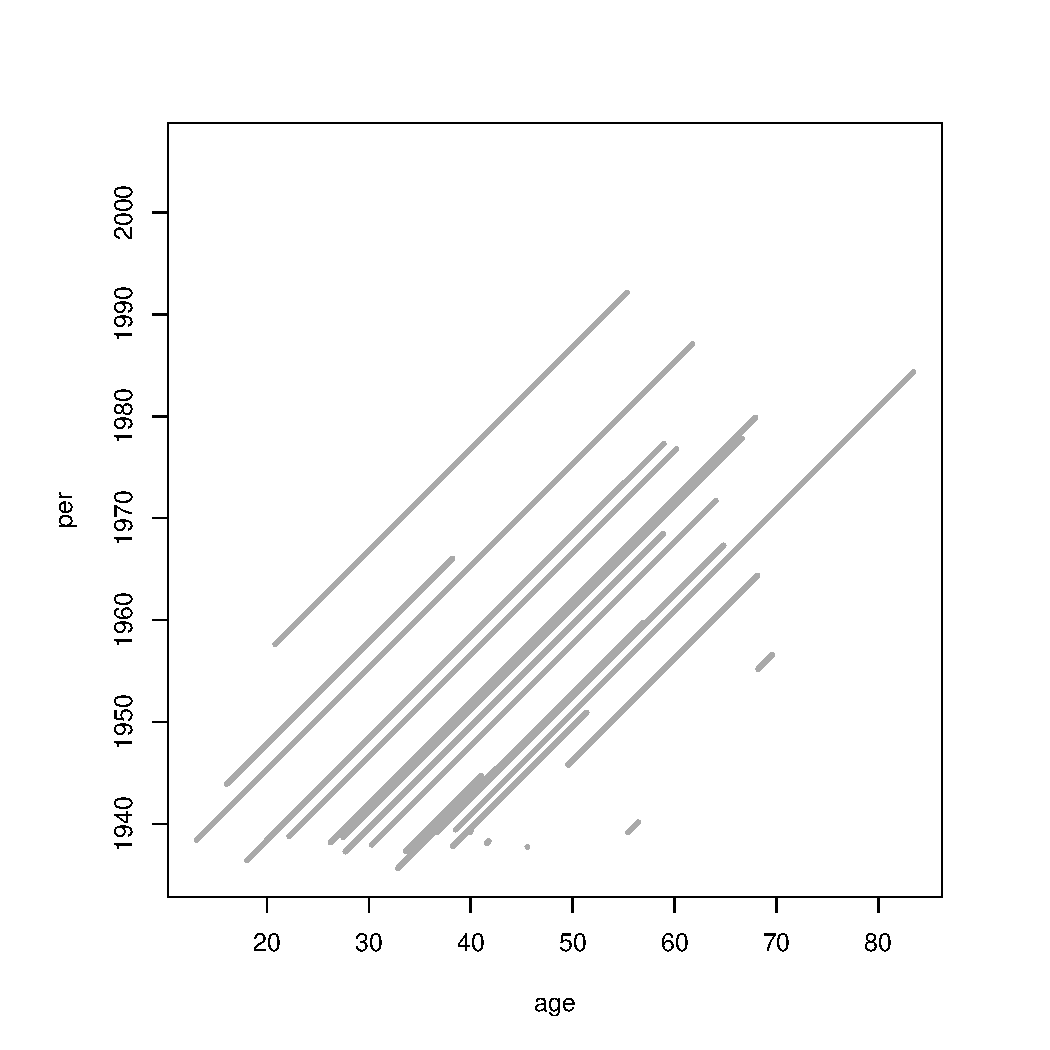
\includegraphics[height=0.90\textheight,keepaspectratio]{thL-lexis0}
{\scriptsize
\begin{verbatim}
> plot( thL, lwd=3 )
\end{verbatim}}
\end{frame}

% %----------------------------------------------------------------------
% \begin{frame}[fragile]
%   \begin{minipage}[c]{0.70\textwidth}
%     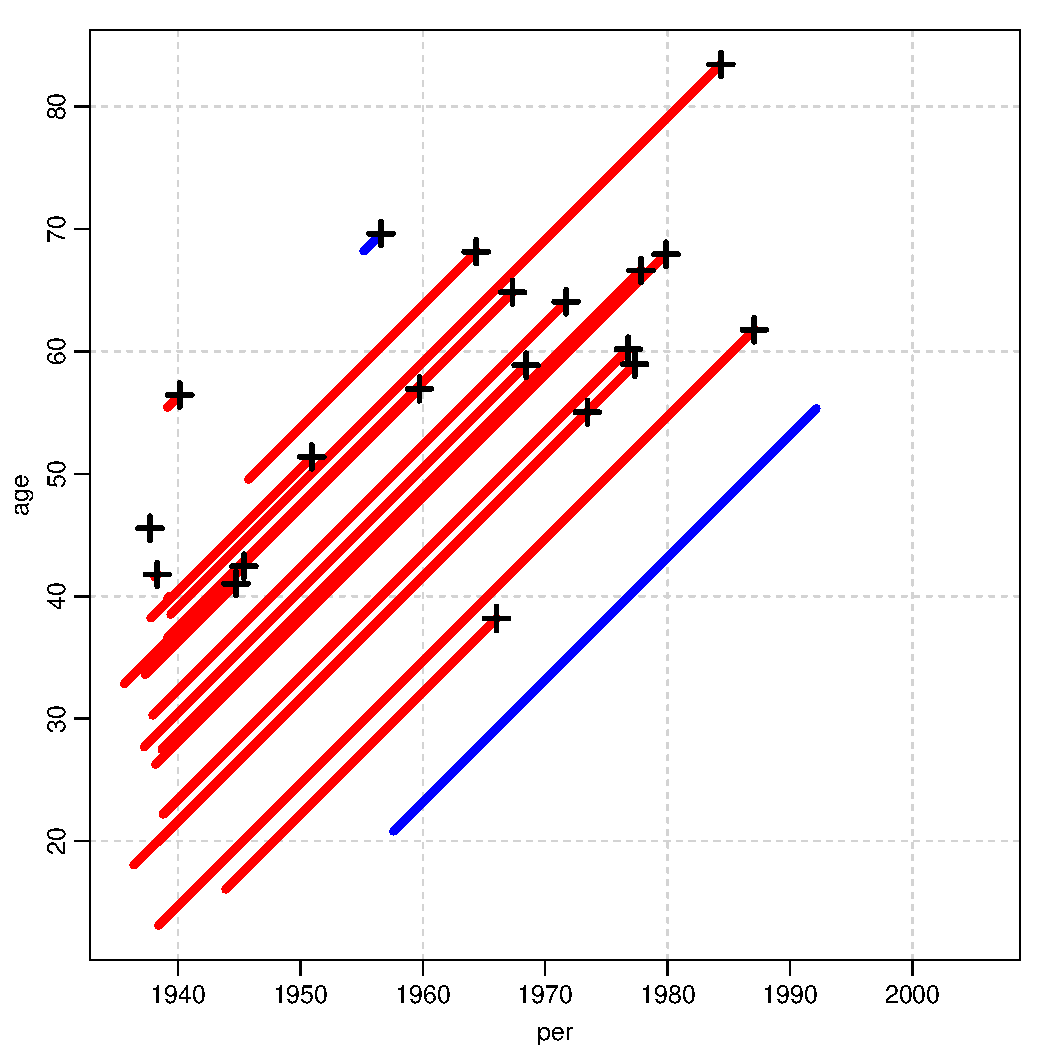
\includegraphics[height=0.85\textheight,keepaspectratio]{thL-lexis1}
%   \end{minipage}
% \hfill
%   \begin{minipage}[c]{0.28\textwidth}
%     Lexis diagram
%   \end{minipage}
% {\scriptsize
% \begin{verbatim}
% > plot( thL, 2:1, lwd=5, col=c("red","blue")[thL$contrast], grid=T )
% > points( thL, 2:1, pch=c(NA,3)[thL$lex.Xst+1],lwd=3, cex=1.5 )
% \end{verbatim}}
% \end{frame}

%----------------------------------------------------------------------
\begin{frame}[fragile]
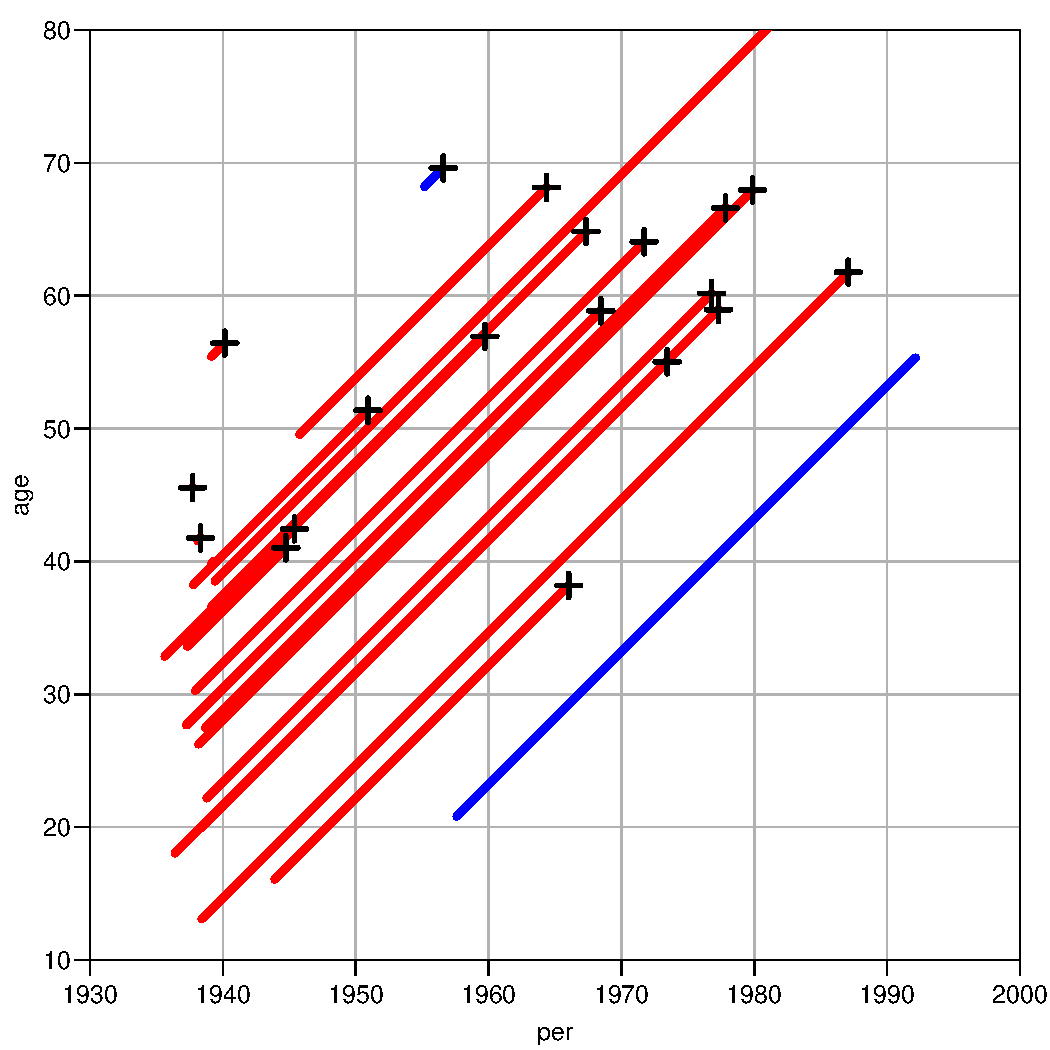
\includegraphics[height=0.80\textheight,keepaspectratio]{thL-lexis2}
\vspace*{-1ex}
{\scriptsize
\begin{verbatim}
> plot( thL, 2:1, lwd=5, col=c("red","blue")[thL$contrast],
+       grid=TRUE, lty.grid=1, col.grid=gray(0.7),
+       xlim=1930+c(0,70), xaxs="i", ylim=  10+c(0,70), yaxs="i", las=1 )
> points( thL, 2:1, pch=c(NA,3)[thL$lex.Xst+1],lwd=3, cex=1.5 )
\end{verbatim}}
\end{frame}

\addtocounter{framenumber}{-1}
%----------------------------------------------------------------------
\begin{frame}[fragile]
  \begin{minipage}[t]{0.60\textwidth}
    \ \\[-1em]
    \hspace*{-2em}
    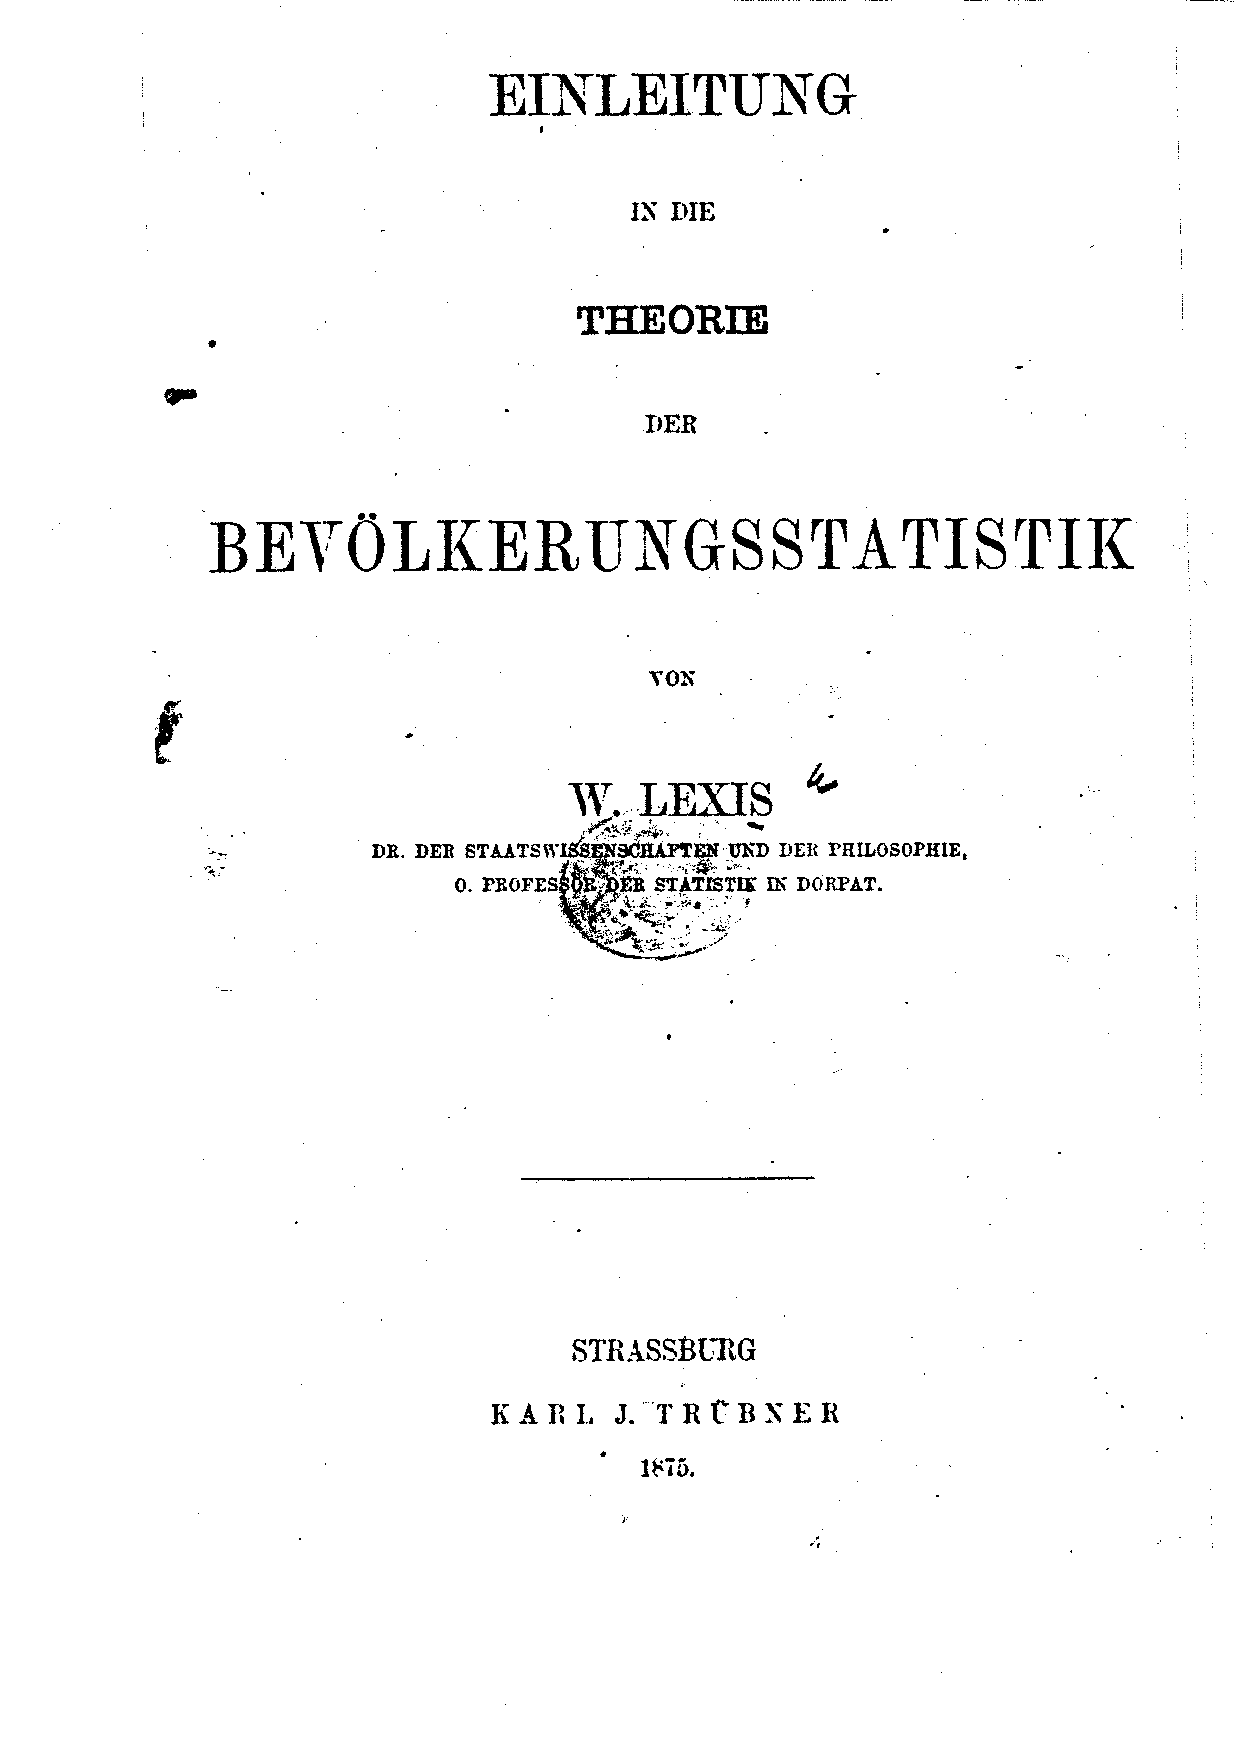
\includegraphics[height=1.5\textheight,keepaspectratio]{Lexis-titlepage}
  \end{minipage}
  \begin{minipage}[t]{0.38\textwidth}
    \ \\[-1ex]
   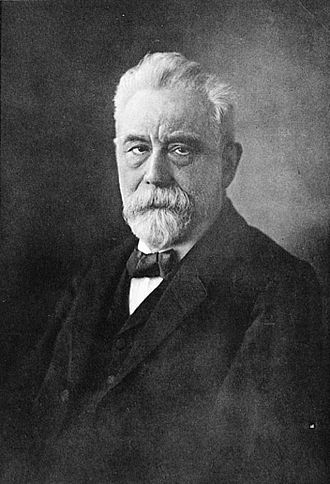
\includegraphics[width=\textwidth,keepaspectratio]{Lexis-portrait}
  \end{minipage}
\end{frame}

%----------------------------------------------------------------------
\begin{frame}[fragile]
  \frametitle{Splitting follow-up time}
\footnotesize
\renewcommand{\baselinestretch}{0.9}
\begin{semiverbatim}
> spl1 <- splitLexis( thL, breaks=seq(0,100,20),
>                          time.scale="age" )
> round(spl1,1)
   age    per  tfi lex.dur lex.Cst lex.Xst   id sex birthdat contrast injecdat volume
\alert<2>{1 22.2 1938.8  0.0    17.8       0       0    1   2   1916.6        1   1938.8     22}
\alert<2>{2 40.0 1956.6 17.8    20.0       0       0    1   2   1916.6        1   1938.8     22}
\alert<2>{3 60.0 1976.6 37.8     0.2       0       1    1   2   1916.6        1   1938.8     22}
\alert<3>{4 49.5 1945.8  0.0    10.5       0       0  640   2   1896.2        1   1945.8     20}
\alert<3>{5 60.0 1956.2 10.5     8.1       0       1  640   2   1896.2        1   1945.8     20}
\alert<4>{6 68.2 1955.2  0.0     1.4       0       1 3425   1   1887.0        2   1955.2      0}
\alert<5>{7 20.8 1957.6  0.0    19.2       0       0 4017   2   1936.8        2   1957.6      0}
\alert<5>{8 40.0 1976.8 19.2    15.3       0       0 4017   2   1936.8        2   1957.6      0}
...
\end{semiverbatim}
\renewcommand{\baselinestretch}{1.0}

\end{frame}

%----------------------------------------------------------------------
\begin{frame}[fragile]
  \frametitle{Split on another timescale}
\vspace*{-1em}
\footnotesize
\renewcommand{\baselinestretch}{0.9}
\begin{semiverbatim}
> spl2 <- splitLexis( spl1, time.scale="tfi",
                            breaks=c(0,1,5,20,100) )
> round( spl2, 1 )
   lex.id  age    per  tfi lex.dur lex.Cst lex.Xst   id sex birthdat contrast injecdat volume
\alert<2>{1       1 22.2 1938.8  0.0     1.0       0       0    1   2   1916.6        1   1938.8     22}
\alert<2,4>{2       1 23.2 1939.8  1.0     4.0       0       0    1   2   1916.6        1   1938.8     22}
\alert<2,4>{3       1 27.2 1943.8  5.0    12.8       0       0    1   2   1916.6        1   1938.8     22}
\alert<2,3>{4       1 40.0 1956.6 17.8     2.2       0       0    1   2   1916.6        1   1938.8     22}
\alert<2,4>{5       1 42.2 1958.8 20.0    17.8       0       0    1   2   1916.6        1   1938.8     22}
\alert<2,3>{6       1 60.0 1976.6 37.8     0.2       0       1    1   2   1916.6        1   1938.8     22}
\alert<5>{7       2 49.5 1945.8  0.0     1.0       0       0  640   2   1896.2        1   1945.8     20}
\alert<5>{8       2 50.5 1946.8  1.0     4.0       0       0  640   2   1896.2        1   1945.8     20}
\alert<5>{9       2 54.5 1950.8  5.0     5.5       0       0  640   2   1896.2        1   1945.8     20}
\alert<5>{10      2 60.0 1956.2 10.5     8.1       0       1  640   2   1896.2        1   1945.8     20}
\alert<6>{11      3 68.2 1955.2  0.0     1.0       0       0 3425   1   1887.0        2   1955.2      0}
\alert<6>{12      3 69.2 1956.2  1.0     0.4       0       1 3425   1   1887.0        2   1955.2      0}
\alert<7>{13      4 20.8 1957.6  0.0     1.0       0       0 4017   2   1936.8        2   1957.6      0}
\alert<7>{14      4 21.8 1958.6  1.0     4.0       0       0 4017   2   1936.8        2   1957.6      0}
\alert<7>{15      4 25.8 1962.6  5.0    14.2       0       0 4017   2   1936.8        2   1957.6      0}
\alert<7>{16      4 40.0 1976.8 19.2     0.8       0       0 4017   2   1936.8        2   1957.6      0}
\alert<7>{17      4 40.8 1977.6 20.0    14.5       0       0 4017   2   1936.8        2   1957.6      0}
...
\end{semiverbatim}
\end{frame}

%----------------------------------------------------------------------
\begin{frame}[fragile]
  \begin{minipage}[t]{0.58\linewidth}
\ \\[-1em] \hspace*{-1em}
\includegraphics[width=\textwidth]<1| handout:1>{thL-lexis2a}
\includegraphics[width=\textwidth]<2| handout:0>{thL-lexis2a1}
\includegraphics[width=\textwidth]<3| handout:0>{thL-lexis2a2}
\includegraphics[width=\textwidth]<4| handout:0>{thL-lexis2a3}
\includegraphics[width=\textwidth]<5| handout:0>{thL-lexis2a4}
\includegraphics[width=\textwidth]<6| handout:0>{thL-lexis2a5}
\includegraphics[width=\textwidth]<7| handout:0>{thL-lexis2a6}
{\scriptsize
\vspace*{-1.5em}
\begin{verbatim}
plot( spl2, c(1,3), col="black", lwd=2 )
\end{verbatim}}
  \end{minipage}
\hfill
  \begin{minipage}[t]{0.37\linewidth}
\footnotesize
\renewcommand{\baselinestretch}{0.9}
\begin{semiverbatim}
 age  tfi lex.dur lex.Cst lex.Xst   id sex birthdat contrast injecdat volume
\alert<2>{22.2  0.0     1.0       0       0    1   2   1916.6        1   1938.8     22}
\alert<3>{23.2  1.0     4.0       0       0    1   2   1916.6        1   1938.8     22}
\alert<4>{27.2  5.0    12.8       0       0    1   2   1916.6        1   1938.8     22}
\alert<5>{40.0 17.8     2.2       0       0    1   2   1916.6        1   1938.8     22}
\alert<6>{42.2 20.0    17.8       0       0    1   2   1916.6        1   1938.8     22}
\alert<7>{60.0 37.8     0.2       0       1    1   2   1916.6        1   1938.8     22}
\end{semiverbatim}
  \end{minipage}
\end{frame}

%----------------------------------------------------------------------
\begin{frame}[fragile]
  \frametitle{Likelihood for a constant rate}
  \begin{itemize}[<+->]
  \item This setup is for a situation where it is assumed that rates are
    constant in each of the intervals.
  \item Each observation in the dataset contributes a term to the
    likelihood.
  \item Each term looks like a contribution from a Possion variate
    (albeit with values only $0$ or $1$)
  \item Rates can vary along several timescales simultaneously.
  \item Models can include fixed covariates, as well as the timescales
    (the left end-points of the intervals) as continuous variables.
  \item The latter is where we will need splines.
  \end{itemize}

\end{frame}

% %----------------------------------------------------------------------
% \begin{frame}[fragile]
%   \frametitle{Likelihood for a constant rate}
% Observation of $D$ cases during $Y$ person-years.
% \begin{center}
% \begin{tabular}{@{\extracolsep{1cm}}cc}
%  $ D\log(\lambda) - \lambda Y $ & $\hat \lambda =
%  \displaystyle\frac{D}{Y}$ \\ \\
% ``Poisson'' likelihood  & M.L. estimate \\
% \end{tabular}
% \end{center}
% \pause
% The log-likelihood for a\\ Poisson variate $D$, with
% mean $\lambda Y$:
% \[
%    D\log(\lambda Y) - \lambda Y =  D\log(\lambda) \onslide<2>{+ D\log(Y)} - \lambda Y
% \]
% \pause
% The term $D\log(Y)$ does not depend on the parameter $\lambda$.
% \end{frame}

% %----------------------------------------------------------------------
% \begin{frame}[fragile]
%   \frametitle{The Poisson likelihood for individual data}

% \[
%    \mbox{L}_\text{cohort}(\lambda | D,Y) \quad \propto \quad
%    \mbox{L}_\text{Poisson}(\lambda Y | D)
% \]

% \pause
% \begin{itemize}[<+->]
% \item $D$ is {\bf not} assumed to be Poisson distributed.
% \item But software that can maximize $\mbox{L}_{\mbox{\scriptsize
%       Poisson}}$ can be used to maximize $\mbox{L}_{\mbox{\scriptsize
%       cohort}}$
% \item The log-link is the canonical link function for the
%   Poisson-distribution, so ``natural'' models are multiplicative
%   models for the mean.
% \end{itemize}

% \end{frame}

% %----------------------------------------------------------------------
% \begin{frame}[fragile]
%   \frametitle{The Poisson likelihood for individual data}
%   \begin{itemize}[<+->]
%   \item The observation from a cohort study is $(D,Y)$:
% \[
%    D = \sum_p d_p, \quad  Y = \sum_p y_p
% \]
% \item Individual records (one per \textbf{p}erson):
% \begin{eqnarray*}
%  D\log(\lambda) - \lambda Y &=&
%  \sum_p d_p\log(\lambda) - \lambda \sum_p y_p \\ &=&
%  \sum_p \left( d_p\log(\lambda) - \lambda y_p \right)
% \end{eqnarray*}
% \item Assuming that the death indicator ($d_p \in \{0,1\}$) is
%   Poisson, with $\log$-offset $y_p$ will give the same result.
%   \end{itemize}
% \end{frame}

%----------------------------------------------------------------------
\begin{frame}[fragile]
  \frametitle{The Poisson likelihood for split data}
\begin{itemize}[<+->]
\item Split records (one per \textbf{p}erson-\textbf{i}nterval
  ($p,i$)):
\[
 \sum_{p,i} \bigl( d_{pi}\log(\lambda) - \lambda y_{pi} \bigr)
 = D\log(\lambda) - \lambda Y
\]
\item Assuming that the death indicator ($d_{pi} \in \{0,1\}$) is Poisson,
  a model with with offset $\log(y_{pi})$ will give the same result.
\item If we assume that rates are constant we get the simple
  expression with $(D,Y)$
\item \ldots but the split data allows models that assume different
  rates for different $(d_{pi},y_{pi})$, so rates can vary
  \textbf{within} a person's follow-up.
\end{itemize}
\end{frame}


%----------------------------------------------------------------------
\begin{frame}[fragile]
  \frametitle{Where is $(d_{pi},y_{pi})$ in the split data?}
\begin{Schunk}
\begin{Sinput}
> spl1 <- splitLexis( thL , breaks=seq(0,100,20)  , time.scale="age" )
> spl2 <- splitLexis( spl1, breaks=c(0,1,5,20,100), time.scale="tfi" )
> options( digits=5 )
> spl2[1:10,1:11]
\end{Sinput}
\begin{Soutput}
   lex.id    age    per    tfi  lex.dur lex.Cst lex.Xst id sex birthdat contrast
1       1 22.182 1938.8  0.000  1.00000       0       0  1   2   1916.6        1
2       1 23.182 1939.8  1.000  4.00000       0       0  1   2   1916.6        1
3       1 27.182 1943.8  5.000 12.81793       0       0  1   2   1916.6        1
4       1 40.000 1956.6 17.818  2.18207       0       0  1   2   1916.6        1
5       1 42.182 1958.8 20.000 17.81793       0       0  1   2   1916.6        1
6       1 60.000 1976.6 37.818  0.17796       0       1  1   2   1916.6        1
7       2 16.063 1943.9  0.000  1.00000       0       0  2   2   1927.8        1
8       2 17.063 1944.9  1.000  2.93703       0       0  2   2   1927.8        1
9       2 20.000 1947.8  3.937  1.06297       0       0  2   2   1927.8        1
10      2 21.063 1948.9  5.000 15.00000       0       0  2   2   1927.8        1
\end{Soutput}
\end{Schunk}
--- and what are covariates for the rates?
\end{frame}

%----------------------------------------------------------------------
\begin{frame}[fragile]
  \frametitle{Analysis of results}
\begin{itemize}[<+->]
\item $d_{pi}$ --- events in the variable: \texttt{lex.Xst}:\\
     In the model as response: \texttt{lex.Xst==1}
\item $y_{pi}$ --- risk time: \texttt{lex.dur} (duration):\\
     In the model as offset $\log(y)$, \texttt{log(lex.dur)}.
\item Covariates are:
\begin{itemize}
\item timescales (age, period, time in study)
\item other variables for this person
(constant or {\em assumed} constant in each interval).
\end{itemize}
\item Model rates using the covariates in \texttt{glm}:\\
  --- no difference between time-scales and other covariates.
\end{itemize}
\end{frame}

% %----------------------------------------------------------------------
% \begin{frame}[fragile]
%   \frametitle{Poisson model for split data}
%   \begin{itemize}[<+->]
%   \item Each interval contribute $\lambda Y$ to the log-likelihood.
%   \item All intervals with the same set of covariate values
%     (age,exposure,\ldots) have the same $\lambda$.
%   \item The log-likelihood contribution from these is $\lambda \sum Y$
%     --- the same as from aggregated data.
%   \item The event intervals contribute each $D \log \lambda$.
%   \item The log-likelihood contribution from those with the same
%     lambda is $\sum D \log \lambda$ --- the same as from aggregated
%     data.
%   \item The log-likelihood is the same for split data and aggregated
%   data --- no need to tabulate first.
%   \end{itemize}
% \end{frame}

%----------------------------------------------------------------------
\begin{frame}[fragile]
  \frametitle{Fitting a simple model}
\begin{Schunk}
\begin{Sinput}
> stat.table( contrast,
+             list( D = sum( lex.Xst ),
+                   Y = sum( lex.dur ),
+                Rate = ratio( lex.Xst, lex.dur, 100 ) ),
+             margin = TRUE,
+             data = spl2 )
\end{Sinput}
\begin{Soutput}
 ------------------------------------ 
 contrast         D        Y    Rate  
 ------------------------------------ 
 1           928.00 20094.74    4.62  
 2          1036.00 31839.35    3.25  
                                      
 Total      1964.00 51934.08    3.78  
 ------------------------------------ 
\end{Soutput}
\end{Schunk}
\end{frame}

%----------------------------------------------------------------------
\begin{frame}[fragile]
  \frametitle{Fitting a simple model}
\begin{Schunk}
\begin{Soutput}
 ------------------------------------ 
 contrast         D        Y    Rate  
 ------------------------------------ 
 1           928.00 20094.74    4.62  
 2          1036.00 31839.35    3.25  
 ------------------------------------ 
\end{Soutput}
\end{Schunk}
\begin{Schunk}
\begin{Sinput}
> m0 <- glm( (lex.Xst==1) ~ factor(contrast) - 1,
+            offset = log(lex.dur/100),
+            family = poisson, 
+              data = spl2 )
> round( ci.exp( m0 ), 2 )
\end{Sinput}
\begin{Soutput}
                  exp(Est.) 2.5% 97.5%
factor(contrast)1      4.62 4.33  4.93
factor(contrast)2      3.25 3.06  3.46
\end{Soutput}
\end{Schunk}
\end{frame}
